\documentclass[reprint,aps,unsortedaddress,superscriptaddress,prd,floatfix,showpacs,linenumbers]{revtex4-2}
\usepackage[utf8]{inputenc}
\usepackage{float}
\usepackage{graphicx}
\usepackage{amsmath,amsthm,amssymb}
\usepackage{verbatim}
\usepackage{url}
\usepackage{subcaption}
\usepackage[separate-uncertainty=true]{siunitx}
\usepackage{physics}
\usepackage{hyperref}
\usepackage[capitalize]{cleveref}
\usepackage[obeyFinal]{todonotes}
\setuptodonotes{inline}
\usepackage{adjustbox}
\usepackage{multirow}
\usepackage{lineno}
\linenumbers
\graphicspath{{figures/}}
\DeclareSIUnit\barn{b}

\captionsetup{justification=raggedright,singlelinecheck=false}

\begin{document}

\title{Improve measurement of flavor asymmetry of the light-quark sea in the proton with Drell-Yan production in
	\texorpdfstring{$p+p$}{p+p} and \texorpdfstring{$p+d$}{p+d} collisions at \texorpdfstring{\SI{120}{\GeV}}{120~GeV}}
% !TeX root = main.tex
\author{C.~H.~Leung}
\affiliation{Department of Physics, University of Illinois at Urbana-Champaign, Urbana, Illinois 61801, USA}

\author{J.~C.~Peng}
\affiliation{Department of Physics, University of Illinois at Urbana-Champaign,
Urbana, Illinois 61801, USA}

\begin{comment}
\author{J. Dove}
\affiliation{Department of Physics, University of Illinois at Urbana-Champaign,
Urbana, Illinois 61801, USA}

\author{B.~Kerns}
\affiliation{Department of Physics, University of Illinois at Urbana-Champaign,
Urbana, Illinois 61801, USA}

\author{R.~E.~McClellan}
\altaffiliation[Present address ]{Pensacola State College, Pensacola, FL 32504}
\affiliation{Department of Physics, University of Illinois at Urbana-Champaign, 
Urbana, Illinois 61801, USA}

\author{S.~Miyasaka}
\affiliation{Department of Physics, Tokyo Institute of Technology, Meguro-ku, Tokyo 152-8550, Japan}

\author{D.~H.~Morton}
\affiliation{Randall Laboratory of Physics, University of Michigan, Ann Arbor,
Michigan 48109, USA}

\author{K.~Nagai}
\affiliation{Department of Physics, Tokyo Institute of Technology, Meguro-ku, Tokyo 152-8550, Japan}
\affiliation{Institute of Physics, Academia Sinica, Taipei, 11529, Taiwan}
\affiliation{Physics Division, Los Alamos National Laboratory, Los Alamos, New Mexico 97545, USA}

\author{S.~Prasad}
\affiliation{Department of Physics, University of Illinois at Urbana-Champaign,
Urbana, Illinois 61801, USA}
\affiliation{Physics Division, Argonne National Laboratory, Lemont, Illinois 60439, USA}

\author{F.~Sanftl}
\affiliation{Department of Physics, Tokyo Institute of Technology, Meguro-ku,
Tokyo 152-8550, Japan}

\author{M.~B.~C.~Scott}
\affiliation{Randall Laboratory of Physics, University of Michigan, Ann Arbor,Michigan 48109, USA}
\affiliation{Physics Division, Argonne National Laboratory, Lemont, Illinois 60439, USA}

\author{A.~S.~Tadepalli}
\altaffiliation[Present address ]{Thomas Jefferson National Accelerator Facility, Newport News, Virginia 23606, USA}
\affiliation{Department of Physics and Astronomy, Rutgers, The State University of New Jersey, Piscataway, New Jersey 08854, USA}

\author{C.~A.~Aidala}
\affiliation{Randall Laboratory of Physics, University of Michigan, Ann Arbor, Michigan 48109, USA}
\affiliation{Physics Division, Los Alamos National Laboratory, Los Alamos, New Mexico 87545, USA}

\author{J.~ Arrington}
\altaffiliation[Present address ]{Lawrence Berkeley National Laboratory, Berkeley, California, 94720 USA}
\affiliation{Physics Division, Argonne National Laboratory, Lemont, Illinois 60439, USA}

\author{C.~Ayuso}
\affiliation{Randall Laboratory of Physics, University of Michigan, Ann Arbor,
Michigan 48109, USA}

\author{C.~T.~Barker}
\affiliation{Department of Engineering and Physics, Abilene Christian University, Abilene, Texas 79699, USA}

\author{C.~N.~Brown}
\affiliation{Fermi National Accelerator Laboratory, Batavia, Illinois 60510, USA}

\author{T.~H.~Chang}
\affiliation{Institute of Physics, Academia Sinica, Taipei, 11529, Taiwan}

\author{W.~C.~Chang}
\affiliation{Institute of Physics, Academia Sinica, Taipei, 11529, Taiwan}

\author{A.~Chen}
\affiliation{Department of Physics, University of Illinois at Urbana-Champaign, Urbana, Illinois 61801, USA}
\affiliation{Institute of Physics, Academia Sinica, Taipei, 11529, Taiwan}
\affiliation{Randall Laboratory of Physics, University of Michigan, Ann Arbor, Michigan 48109, USA}

\author{D.~C.~Christian}
\affiliation{Fermi National Accelerator Laboratory, Batavia, Illinois 60510, USA}

\author{B.~P.~Dannowitz}
\affiliation{Department of Physics, University of Illinois at Urbana-Champaign, Urbana, Illinois 61801, USA}

\author{M.~Daugherity}
\affiliation{Department of Engineering and Physics, Abilene Christian University, Abilene, Texas 79699, USA}

\author{M.~Diefenthaler}
\affiliation{Department of Physics, University of Illinois at Urbana-Champaign, Urbana, Illinois 61801, USA}

\author{L.~El Fassi}
\affiliation{Department of Physics and Astronomy, Mississippi State University, Mississippi State, Mississippi 39762, USA }
\affiliation{Department of Physics and Astronomy, Rutgers, The State University of New Jersey, Piscataway, New Jersey 08854, USA}

\author{D.~F.~Geesaman}
\affiliation{Physics Division, Argonne National Laboratory, Lemont, Illinois 60439, USA}

\author{R.~Gilman}
\affiliation{Department of Physics and Astronomy, Rutgers, The State University of New Jersey, Piscataway, New Jersey 08854, USA}

\author{Y.~Goto}
\affiliation{RIKEN Nishina Center for Accelerator-Based Science, Wako, Saitama 351-0198, Japan}

\author{L.~Guo}
\altaffiliation[Present address ]{Florida International University, Miami, Florida, 33199, USA}
\affiliation{Physics Division, Los Alamos National Laboratory, Los Alamos, New Mexico 87545, USA}

\author{R.~Guo}
\affiliation{Department of Physics, National Kaohsiung Normal University, Kaohsiung City 80201, Taiwan}

\author{T.~J.~Hague}
\altaffiliation[Present address ]{Lawrence Berkeley National Laboratory, Berkeley, California, 94720 USA}
\affiliation{Department of Engineering and Physics, Abilene Christian University, Abilene, Texas 79699, USA}

\author{R.~J.~Holt}
\altaffiliation[Present address ]{Kellogg Radiation Laboratory, California Institute of Technology, Pasadena, California 91125, USA}
\affiliation{Physics Division, Argonne National Laboratory, Lemont, Illinois 60439, USA}

\author{D.~Isenhower}
\affiliation{Department of Engineering and Physics, Abilene Christian University, Abilene, Texas 79699, USA}

\author{E.~R.~Kinney}
\affiliation{Department of Physics, University of Colorado, Boulder,
Colorado 80309, USA}

\author{N.~D.~Kitts}
\affiliation{Department of Engineering and Physics, Abilene Christian University, Abilene, Texas 79699, USA}

\author{A.~Klein}
\affiliation{Physics Division, Los Alamos National Laboratory, Los Alamos, New Mexico 87545, USA}

\author{D.~W.~Kleinjan}
\affiliation{Physics Division, Los Alamos National Laboratory, Los Alamos, New Mexico 87545, USA}

\author{Y.~Kudo}
\affiliation{Department of Physics, Yamagata University, Yamagata City, Yamagata 990-8560, Japan}

\author{P.-J.~Lin}
\affiliation{Department of Physics, University of Colorado, Boulder, Colorado 80309, USA}
\affiliation{Institute of Physics, Academia Sinica, Taipei, 11529, Taiwan}

\author{K.~Liu}
\affiliation{Physics Division, Los Alamos National Laboratory, Los Alamos, New Mexico 87545, USA}

\author{M.~X.~Liu}
\affiliation{Physics Division, Los Alamos National Laboratory, Los Alamos,
New Mexico 87545, USA}

\author{W.~Lorenzon}
\affiliation{Randall Laboratory of Physics, University of Michigan, Ann Arbor,
Michigan 48109, USA}

\author{N.~C.~R.~Makins}
\affiliation{Department of Physics, University of Illinois at Urbana-Champaign, Urbana, Illinois 61801, USA}

\author{M.~Mesquita de Medeiros}
\affiliation{Physics Division, Argonne National Laboratory, Lemont,
Illinois 60439, USA}

\author{P.~L.~McGaughey}
\affiliation{Physics Division, Los Alamos National Laboratory, Los Alamos,
New Mexico 87545, USA}

\author{Y.~Miyachi}
\affiliation{Department of Physics, Yamagata University, Yamagata City,
Yamagata 990-8560, Japan}

\author{I.~Mooney}
\altaffiliation[Present address ]{Wayne State University, Detroit, MI 48202, USA}
\affiliation{Randall Laboratory of Physics, University of Michigan, Ann Arbor, Michigan 48109, USA}

\author{K.~Nakahara}
\altaffiliation[Present address ]{Stanford Linear Accelerator Center, Menlo Park, CA 94025, USA}
\affiliation{Department of Physics, University of Maryland, College Park, Maryland 20742, USA}

\author{K.~Nakano}
\affiliation{University of Virginia, Charlottesville, Virginia 22904, USA}
\affiliation{Department of Physics, Tokyo Institute of Technology, Meguro-ku, Tokyo 152-8550, Japan}
\affiliation{RIKEN Nishina Center for Accelerator-Based Science, Wako, Saitama 351-0198, Japan}

\author{S.~Nara}
\affiliation{Department of Physics, Yamagata University, Yamagata City, Yamagata 990-8560, Japan}


\author{A.~J.~Puckett}
\altaffiliation[Present address ]{University of Connecticut, Storrs, CT 06269, USA}
\affiliation{Physics Division, Los Alamos National Laboratory, Los Alamos, New Mexico 87545, USA}

\author{B.~J.~Ramson}
\affiliation{Randall Laboratory of Physics, University of Michigan, Ann Arbor, Michigan 48109, USA}
\affiliation{Fermi National Accelerator Laboratory, Batavia, Illinois 60510, USA}

\author{P.~E.~Reimer}
\affiliation{Physics Division, Argonne National Laboratory, Lemont, Illinois 60439, USA}

\author{J.~G.~Rubin}
\affiliation{Randall Laboratory of Physics, University of Michigan, Ann Arbor, Michigan 48109, USA}
\affiliation{Physics Division, Argonne National Laboratory, Lemont, Illinois 60439, USA}

\author{S.~Sawada}
\affiliation{Institute of Particle and Nuclear Studies, KEK, High Energy Accelerator Research Organization, Tsukuba, Ibaraki 305-0801, Japan}

\author{T.~Sawada}
\altaffiliation[Present address ]{Nambu Yoichiro Institute of Theoretical and Experimental Physics, Osaka Metropolitan University, Osaka 558-8585, JAPAN}
\affiliation{Randall Laboratory of Physics, University of Michigan, Ann Arbor, Michigan 48109, USA}

\author{T.-A.~Shibata}
\altaffiliation[Present address ]{Nihon University, College of Science and Technology, Chiyoda-ku, Tokyo 101-8308, Japan}
\affiliation{Department of Physics, Tokyo Institute of Technology, Meguro-ku, Tokyo 152-8550, Japan}
\affiliation{RIKEN Nishina Center for Accelerator-Based Science, Wako, Saitama 351-0198, Japan}

\author{S.~H.~Shiu}
\affiliation{Institute of Physics, Academia Sinica, Taipei, 11529, Taiwan}

\author{D.~Su}
\affiliation{Institute of Physics, Academia Sinica, Taipei, 11529, Taiwan}

\author{M.~Teo}
\affiliation{Department of Physics, University of Illinois at Urbana-Champaign, Urbana, Illinois 61801, USA}

\author{B.~G Tice}
\affiliation{Physics Division, Argonne National Laboratory, Lemont, Illinois 60439, USA}

\author{R.~S.~Towell}
\affiliation{Department of Engineering and Physics, Abilene Christian University, Abilene, Texas 79699, USA}

\author{S.~Uemura}
\altaffiliation[Present address ]{Fermi National Accelerator Laboratory, Batavia, Illinois 60510, USA}
\affiliation{Department of Engineering and Physics, Abilene Christian University, Abilene, Texas 79699, USA}

\author{T.~S.~Watson}
\affiliation{Department of Engineering and Physics, Abilene Christian University, Abilene, Texas 79699, USA}

\author{S.~G.~Wang}
\altaffiliation[Present address ]{APS, Argonne National Laboratory, Lemont, Illinois 60439, USA}
\affiliation{Institute of Physics, Academia Sinica, Taipei, 11529, Taiwan}
\affiliation{Department of Physics, National Kaohsiung Normal University, Kaohsiung City 80201, Taiwan}

\author{A.~B.~Wickes}
\affiliation{Physics Division, Los Alamos National Laboratory, Los Alamos,
New Mexico 87545, USA}

\author{J.~Wu}
\affiliation{Fermi National Accelerator Laboratory, Batavia, Illinois 60510, USA}

\author{Z.~Xi}
\affiliation{Department of Engineering and Physics, Abilene Christian University, Abilene, Texas 79699, USA}

\author{Z.~Ye}
\altaffiliation[Present address ]{Department of Physics, Tsinghua University, Beijing 100084 China}
\affiliation{Physics Division, Argonne National Laboratory, Lemont, Illinois 60439, USA}
\end{comment}
\author{Others...}
\collaboration{FNAL E906/SeaQuest Collaboration}
%\noaffiliation


\date{\today}

\begin{abstract}
\end{abstract}


\maketitle

\section{Introduction}
\todo{are we comparing with E866 here?}
\todo{summarized previos finding?}
\todo{discribe the results from STAR and why this new result is better}

The results based on Run 2-3 have previously reported~\cite{dove2021,dove2023}. 
In this letter, we report the improved results using all data collected by the SeaQuest Experiment at Fermilab.
The data constitute a twofold increase in the detected muons compared to our previous publications.
\todo{also summarized any improvement in the analysis if any}

\section{The Drell-Yan Process}

\section{The SeaQuest Experiment}
\subsection{Target System}
\subsection{Spectrometer}
\subsection{Trigger System}

\section{Data Analysis}
\todo{progress between nature paper and now?}
\subsection{Track reconstruction}

\subsection{Monte Carlo simulation}
\todo{Explain the event generation, geat4 options, embeding(?), realization(?).}
\todo{How well is our data discribed by GMC? Which distributions are we comparing?}

\subsection{Mass-fit method}
\todo{Explain the method. If we are using NMSU mix, we will need to justify the normalization.}
\begin{figure}[htbp!]
	\centering
	\begin{subfigure}{\linewidth}
		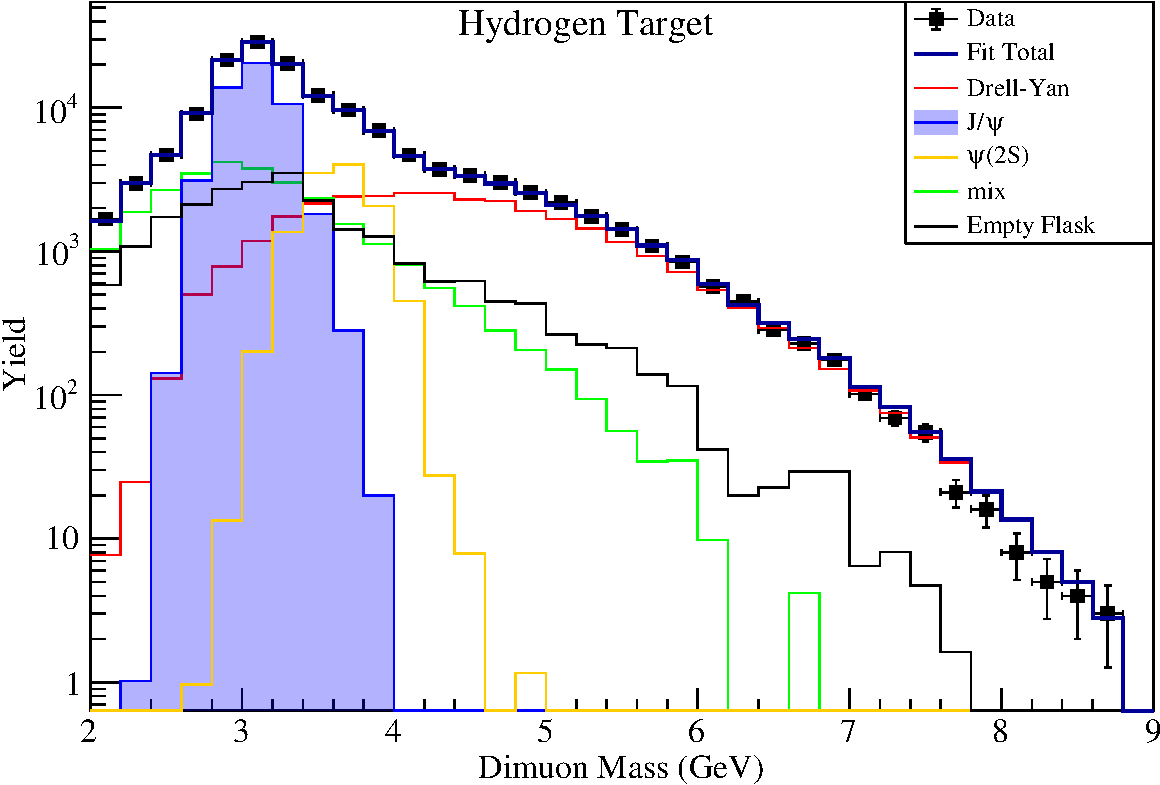
\includegraphics[width=\linewidth]{massfit_run56_LH2.pdf}
	\end{subfigure}
	\begin{subfigure}{\linewidth}
		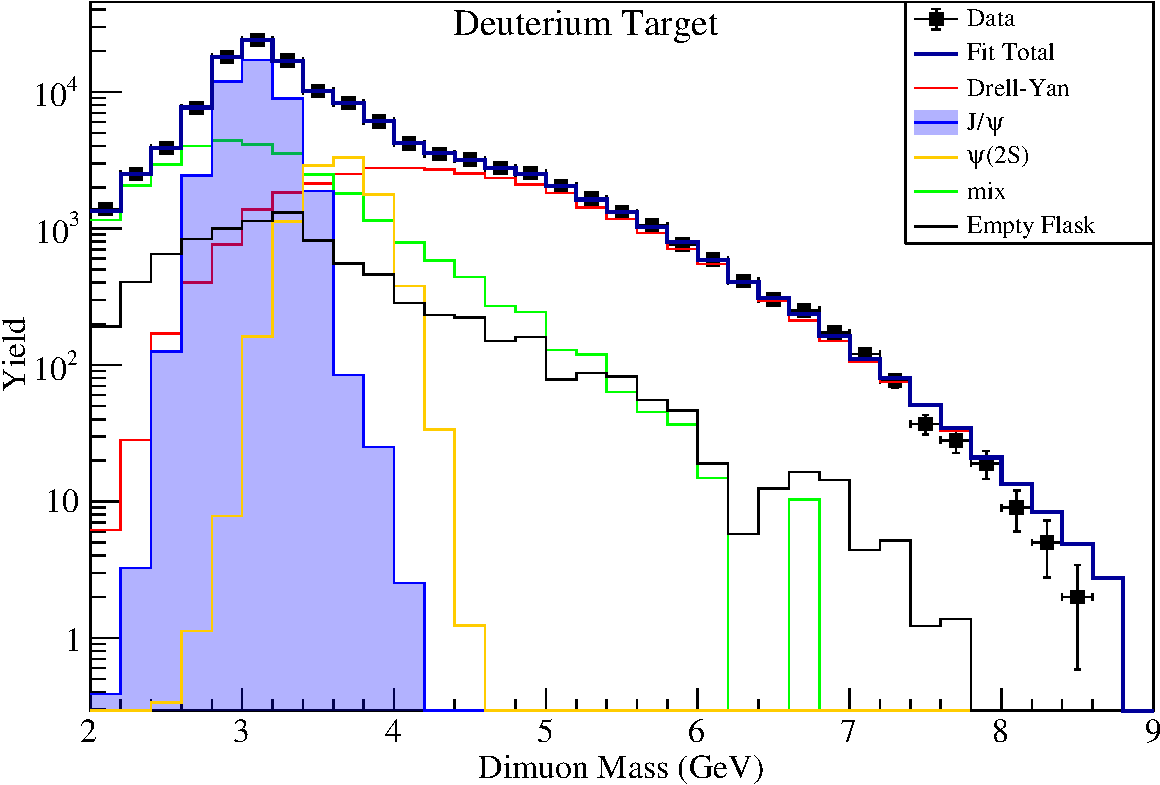
\includegraphics[width=\linewidth]{massfit_run56_LD2.pdf}
	\end{subfigure}
	\caption{Dimuon mass distribution for events collected
	on liquid hydrogen (top) and deuterium (bottom) targets for the second data set.
	The data points (solid squares) are compared with a fit (solid blue line) consisting of
	various components (see text).}
	\label{fig:massfit}
\end{figure}
\missingfigure[figwidth=\linewidth]{Drell-Yan yeild vs $x_T$ after background subtraction compared with MC} 
\todo{corrections(?): rate dependence, target contamination, live PoT}

\section{Measurement of The \texorpdfstring{$\sigma^{pd}/2\sigma^{pp}$}{pd/2pp} Drell-Yan Cross Section Ratio}
\todo{which variables do we want to show? (x2, x1, mass, pT, xF, etc)}
\begin{figure}[htbp!]
	\centering
	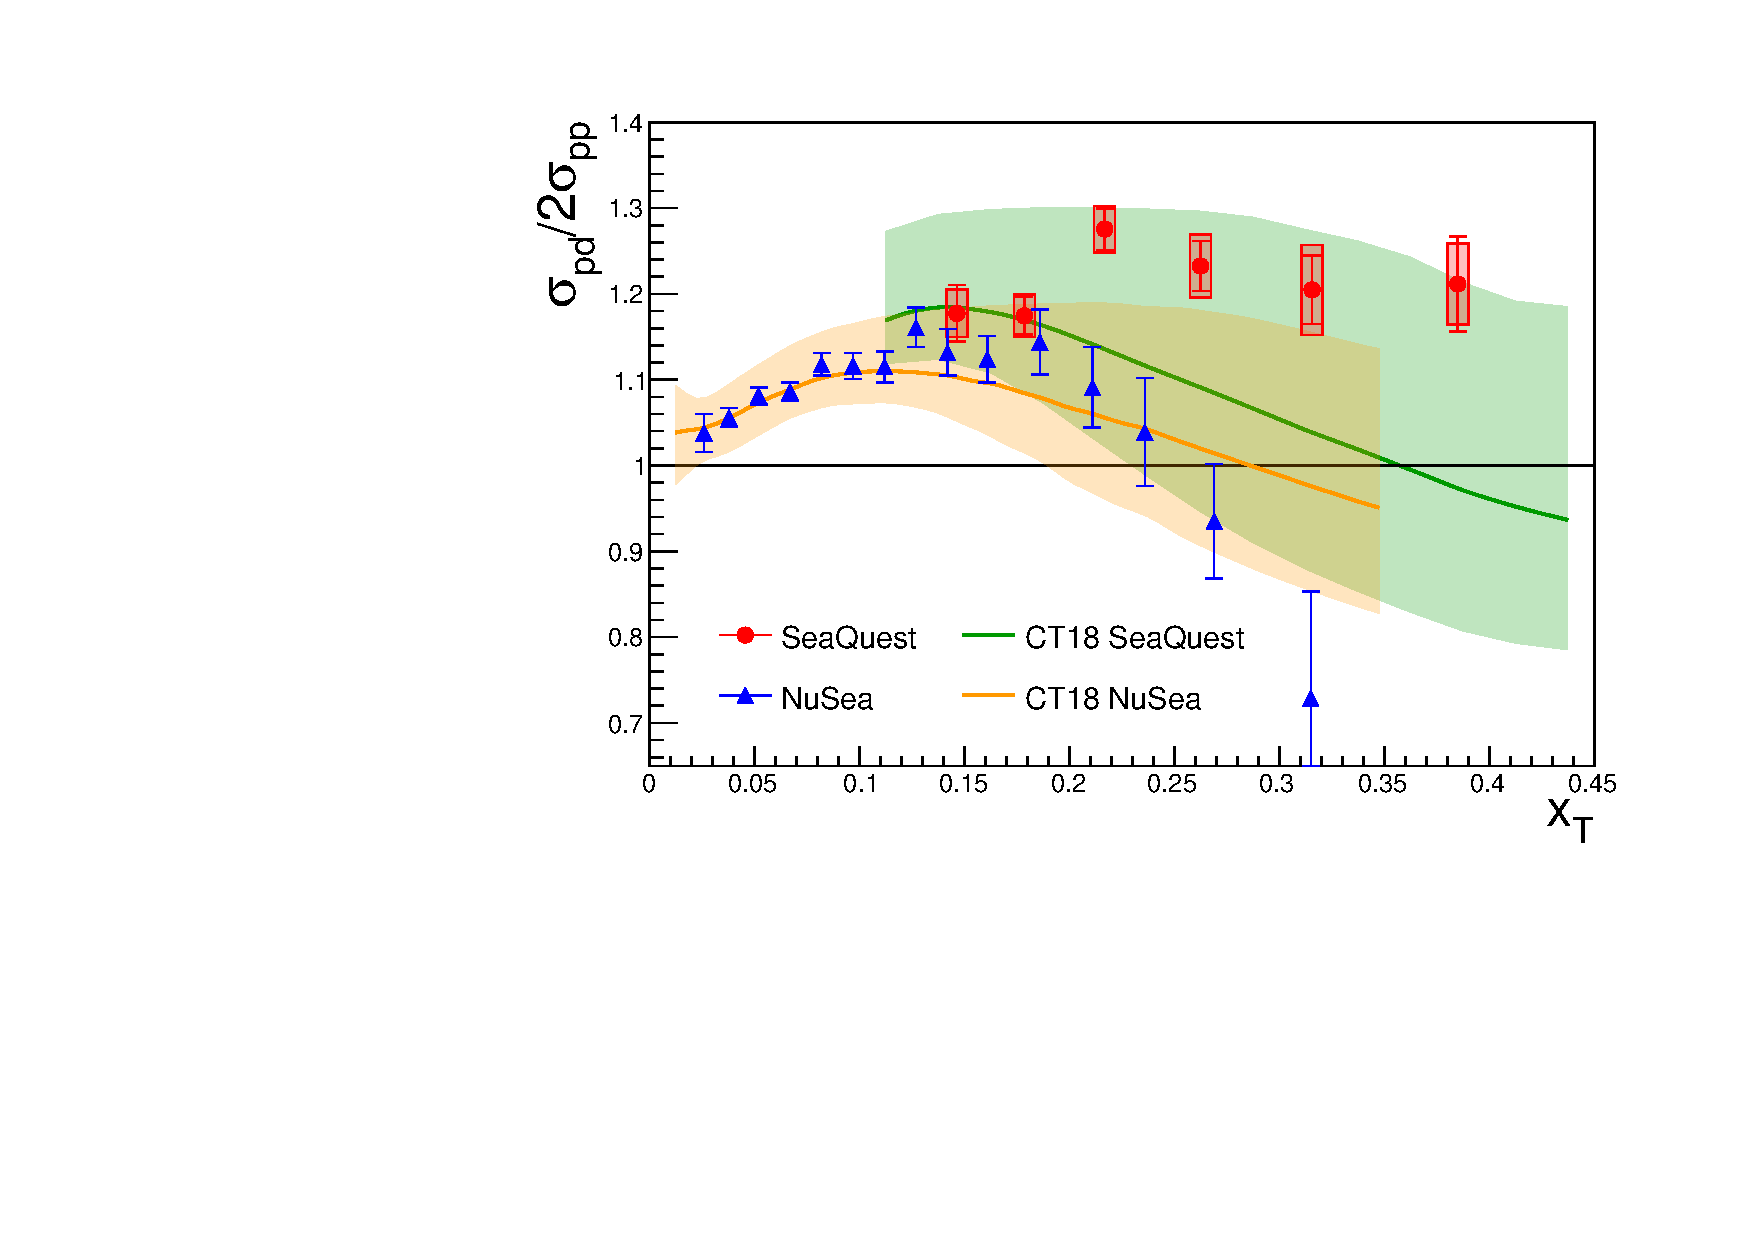
\includegraphics[width=\linewidth]{E906_E866_xT_CT18only.pdf}
	\caption{Measured $\sigma_{pd}/2\sigma_{pp}$ Drell-Yan cross section ratio from SeaQuest compared with E866/NuSea~\cite{towell2001}
		and calculations using CT18~\cite{hou2021} at different kinematics.}
	\label{fig:xT_csr}
\end{figure}

\todo{break down of systematics}
\todo{consistence of the data(source of systematics)}

\section{Extraction of \texorpdfstring{$\bar{d}\left(x\right)/\bar{u}\left(x\right)$}{dbar(x)/ubar(x)}
	and \texorpdfstring{$\bar{d}\left(x\right)-\bar{u}\left(x\right)$}{dbar(x)-ubar(x)}}
\todo{Explain the extraction. There are also addition systematics here.}
\todo{Where to put acceptance? We did show the acceptance in nature paper.}
\begin{figure}[htbp!]
	\centering
	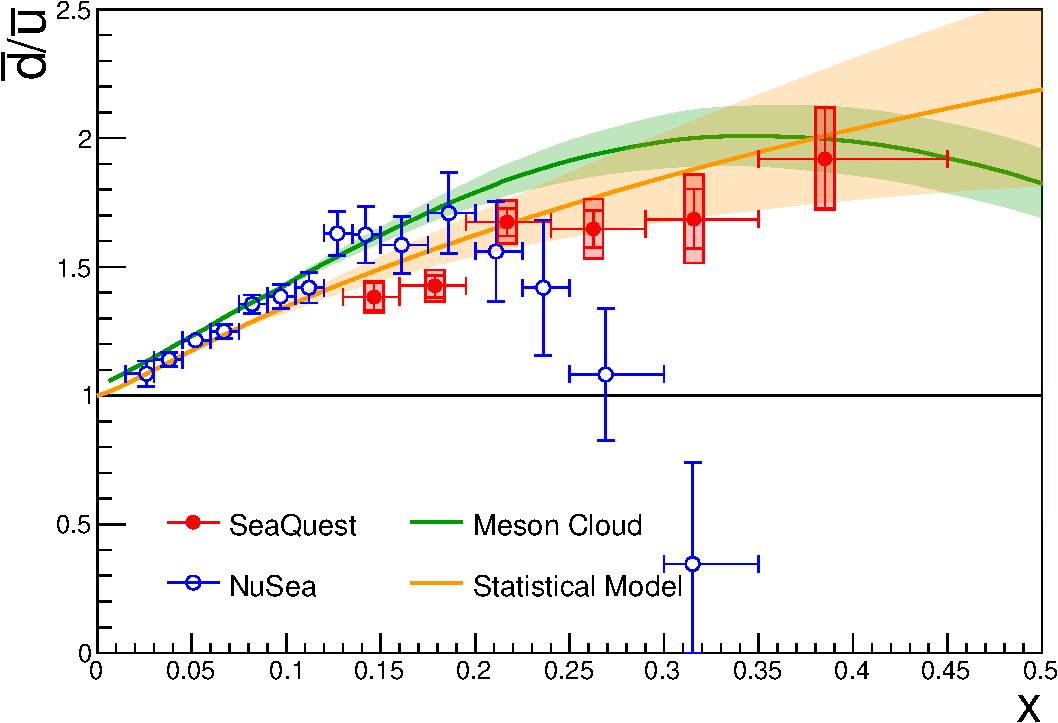
\includegraphics[width=\linewidth]{E906_E866_dbarubar}
	\caption{Comparison of the extracted $\bar{d}\left(x\right)/\bar{u}\left(x\right)$ from SeaQuest
		compared with E866/NuSea~\cite{towell2001} and meson cloud~\cite{alberg2022} and statistical models~\cite{soffer2019}.}
	\label{fig:dbub_ratio}
\end{figure}
\begin{table*}[htbp!]
	\centering
	\caption{The measured $\sigma_{pd}/2\sigma_{pp}$ cross section ratio as well
		as the extracted $\bar{d}/\bar{u}$ and $\bar{d}-\bar{u}$ for each $x_{2}$ bin.
		The first uncertainty is statistical and the second systematic.}
	\begin{adjustbox}{max width=\textwidth}
		% !TeX root = ../main.tex
{
\renewcommand{\arraystretch}{1.5}
\begin{tabular}{cccccccc}
	\hline\hline
	$x_{2}$ range    & $\expval{x_{2}}$ & $\expval{x_{1}}$ & $\expval{p_{T}}(\unit{\GeV/c})$ & $\expval{M}(\unit{\GeV/c^2})$ & $\sigma_{pd}/2\sigma_{pp}$ & $\bar{d}/\bar{u}$                     & $\bar{d}-\bar{u}$                     \\ \hline
	$0.130$--$0.160$ & $0.146$          & $0.687$          & $0.760$                         & $4.71$                        & $1.177\pm0.033\pm0.028$    & $1.383^{+0.058+0.060}_{-0.053-0.060}$ & $0.176^{+0.021+0.024}_{-0.022-0.023}$ \\
	$0.161$--$0.201$ & $0.181$          & $0.610$          & $0.759$                         & $4.87$                        & $1.174\pm0.022\pm0.025$    & $1.431^{+0.041+0.061}_{-0.051-0.061}$ & $0.111^{+0.011+0.011}_{-0.011-0.011}$ \\
	$0.202$--$0.242$ & $0.222$          & $0.553$          & $0.760$                         & $5.11$                        & $1.275\pm0.024\pm0.027$    & $1.672^{+0.052+0.082}_{-0.052-0.082}$ & $0.092^{+0.012+0.012}_{-0.012-0.012}$ \\
	$0.243$--$0.293$ & $0.263$          & $0.516$          & $0.761$                         & $5.44$                        & $1.232\pm0.029\pm0.037$    & $1.653^{+0.073+0.123}_{-0.073-0.113}$ & $0.043^{+0.003+0.013}_{-0.003-0.013}$ \\
	$0.294$--$0.354$ & $0.324$          & $0.492$          & $0.762$                         & $5.83$                        & $1.205\pm0.040\pm0.052$    & $1.694^{+0.124+0.174}_{-0.114-0.174}$ & $0.024^{+0.004+0.004}_{-0.004-0.004}$ \\
	$0.355$--$0.455$ & $0.395$          & $0.474$          & $0.762$                         & $6.34$                        & $1.212\pm0.055\pm0.047$    & $1.925^{+0.205+0.205}_{-0.195-0.205}$ & $0.015^{+0.005+0.005}_{-0.005-0.005}$ \\ \hline\hline
\end{tabular}
}

	\end{adjustbox}
\end{table*}
\begin{table*}[htbp!]
	\centering
	\caption{Values of $\int_{0.45}^{0.13} \left[\bar{d}\left(x\right) - \bar{u}\left(x\right)\right] \dd{x}$
		and $\int_{0.45}^{0.13} x\left[\bar{d}\left(x\right) - \bar{u}\left(x\right)\right] \dd{x}$ at $Q^2=\SI{25.5}{\GeV\squared}$ extracted from
		SeaQuest compared with CT18, NNPDF4.0 PDFs as well as meson cloud and statistical models.}	
	\begin{adjustbox}{max width=\textwidth}
		% !TeX root = ../main.tex
\renewcommand{\arraystretch}{1.5}
\begin{tabular}{ccccccc}
\hline \hline
 &          & \multicolumn{2}{c}{PDFs} & & \multicolumn{2}{c}{Models} \\ \cline{3-4} \cline{6-7}
 & SeaQuest &CJ22     & NNPDF4.0     & & Stat.     & Meson cloud    \\ \hline
$\int^{0.45}_{0.13} \left[\bar{d}\left(x\right) - \bar{u}\left(x\right) \right]\dd{x}$ &
  $0.0179_{-0.0018}^{+0.0017} {}_{-0.0023}^{+0.0022}$ &
  $0.0167^{+0.0009}_{-0.0028}$ &
  $0.0208^{+0.0036}_{-0.0036}$ & &
  $0.0186$ &
  $0.0180$ \\
$\int^{0.45}_{0.13} x\left[\bar{d}\left(x\right) - \bar{u}\left(x\right) \right]\dd{x}$ &
  $0.00368_{-0.00036}^{+0.00034} {}_{-0.00049}^{+0.00045}$ &
  $0.00319^{+0.00019}_{-0.00063}$ &
  $0.00414^{+0.00078}_{-0.00078}$ & &
  $0.00386$ &
  $0.00361$ \\ \hline \hline
\end{tabular}

	\end{adjustbox}
\end{table*}
\section{Impact on PDF analysis}
\todo{Not sure about this part}

\section{Conclusions}

\begin{acknowledgments}
\todo{Add funding information}
\end{acknowledgments}
\bibliography{reference}

\end{document}

